\documentclass{beamer}
\usepackage{physics, amsmath, amsfonts,amssymb}

\usetheme{Madrid}
\title[]{Bayesian Inference and Information based model check of Langevin Systems}
\author[Sabarno Saha]{Sabarno Saha \inst{1} \and Dr. Rajesh Singh \inst{2}}
\institute[IISERK]{\inst{1} Department of Physical Sciences IISERK \and %
                      \inst{2} Department of Physical Sciences IIT Madras}
\date{\today}

\begin{document}

\frame{\titlepage}

\begin{frame}
  \frametitle{Introduction}
  \begin{enumerate}
    \item Stochastic Thermodynamics
      \begin{itemize}
        \item Stochastic Processes
        \item Brownian Motion
        \item Stochastic Differential equation 
        \item Stochastic Integrals
        \item Langevin Equation 
        \item Fokker-Planck Equation
        \item Euler-Maruyuma Integrator
      \end{itemize}
    \item Bayesian Inference
      \begin{itemize}
        \item Bayes Theorem
        \item Prior Assignment
        \item Example
      \end{itemize}
  \end{enumerate}
\end{frame}

\begin{frame}
  \frametitle{Introduction(Contd.)}
  \begin{enumerate}\setcounter{enumi}{3}
    \item Information Theory
      \begin{itemize}
        \item Shannon Information
        \item Fisher Information
        \item Kullback Liebler Divergence
      \end{itemize}
    \item Nested Sampling
      \begin{itemize}
        \item Likelihood Function
        \item MCMC
        \item Evidence Calculation
      \end{itemize}
    \item Model Check
      \begin{itemize}
        \item Information check
        \item Scaling of Steps
        \item p-value check
      \end{itemize}
  \end{enumerate}

\end{frame}

\begin{frame}
  \frametitle{Stochastic Thermodynamics}
  \begin{definition}

    A stochastic process is a sequence of random variables where the indexing of the variables
    often carries the notion of time.

  \end{definition}
  For example, we have Brownian motion, which is represented using the Wiener process
  (a stochastic process).
  \begin{definition}
    A Wiener process $\hat{W}$ is a stochastic process which has the following conditional pdf
    \begin{displaymath}
      P(\hat{W}(t+\Delta t)=x | \hat{W}(t)=x') = \frac{1}{\sqrt{2 \pi \Delta t}}\exp(-\frac{(x-x')^2}{2 \Delta t})
    \end{displaymath}

  \end{definition}
  The initial conditions are $P(\hat{W}(0) = x) = \delta(x)$ where $\delta(x)$ is the Dirac Delta
  function.
\end{frame}

\begin{frame}
  \frametitle{Stochastic Thermodynamics : Wiener Process}
  \begin{figure}
    \begin{center}
      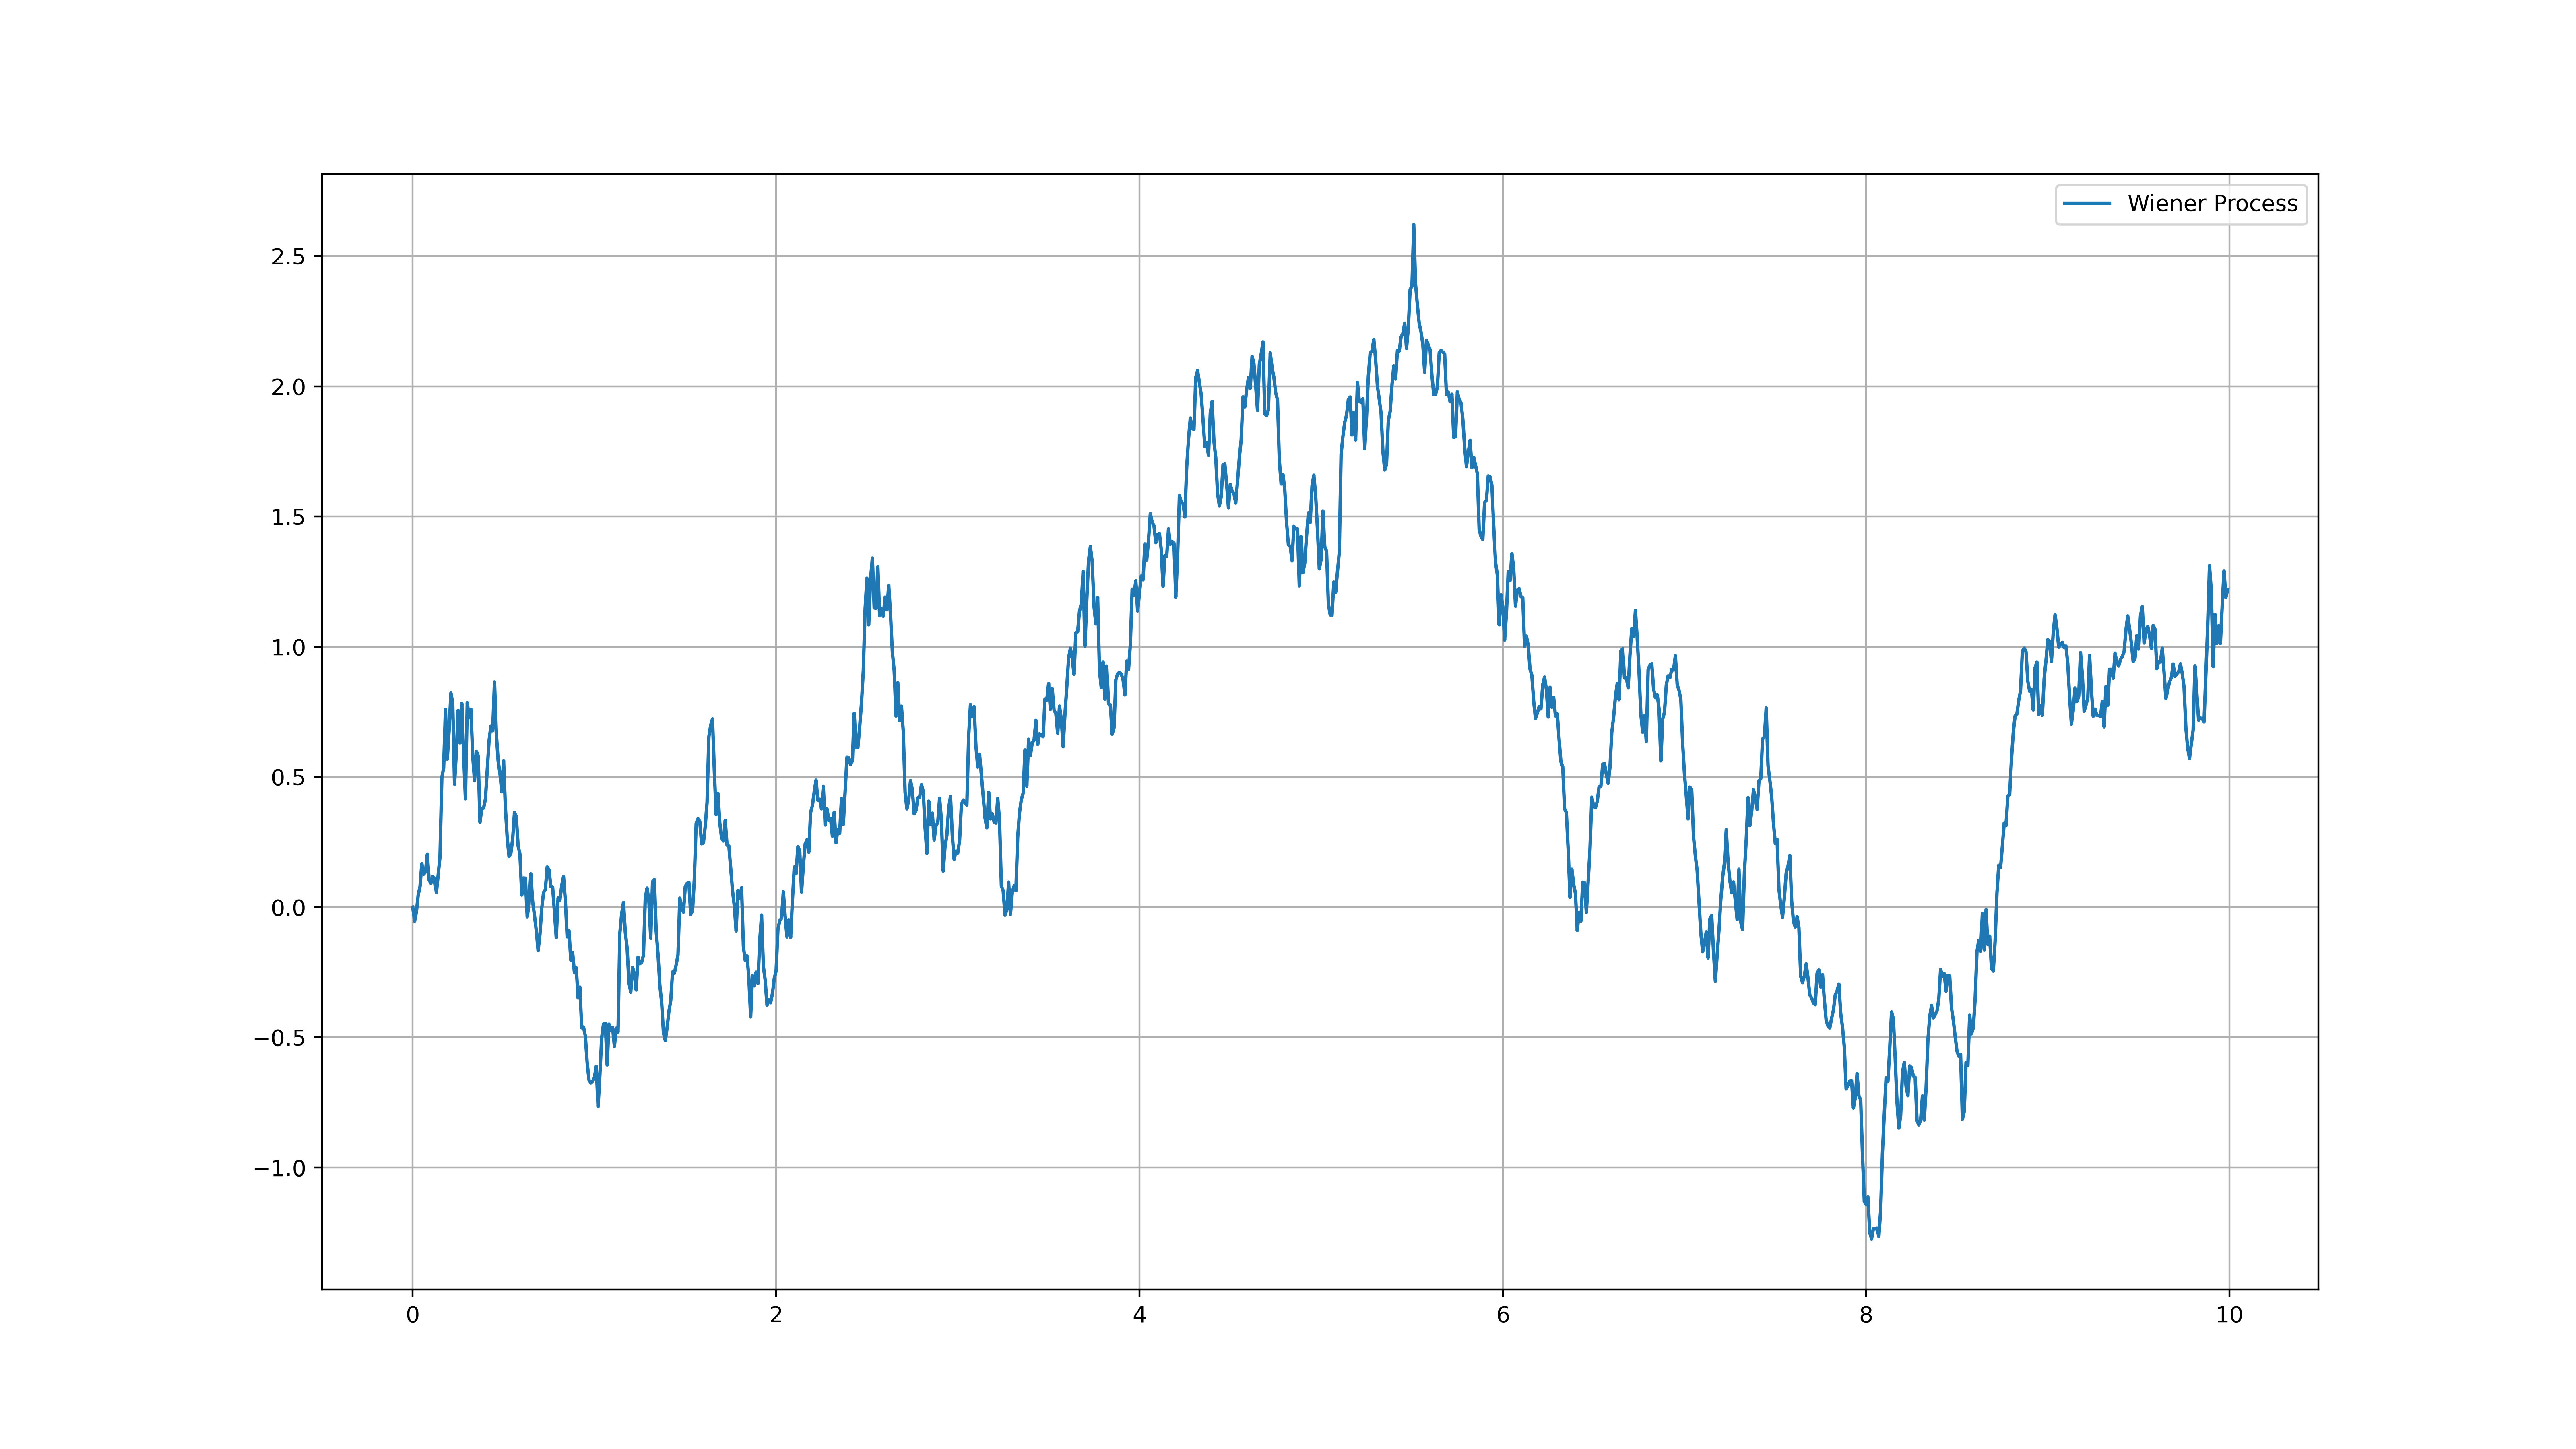
\includegraphics[width=0.95\textwidth]{"../code/WienerProcess.png"}
    \end{center}
    \caption{Wiener Process}\label{fig:1}
  \end{figure}
  
\end{frame}

\begin{frame}
  \frametitle{Stochastic Thermodyamics : Noise}
  \begin{definition}
    The White Gaussian noise $\hat{\xi}(x)$ is defined as 
    \begin{displaymath}
      \lim_{\Delta t \rightarrow 0} \frac{\hat{W}(t+\Delta t)-\hat{W}(t)}{\Delta t}
    \end{displaymath}
  \end{definition}
  \begin{definition}
    The White Gaussian noise $\hat{\xi}(x)$ is also defined as any random variable that has the 
    following properties
      \begin{itemize}
        \item $\mathbb{E}_{t}[\hat{\xi}(t)] = 0$
        \item $\mathbb{E}_{t}[\hat{\xi}(t')\hat{\xi}(t)] \propto \delta (t-t')$
    \end{itemize}
  \end{definition}
  We can have other types of noise as well like telegraphic noise, which we'll see briefly at the 
  very end.
\end{frame}
\begin{frame}
  \frametitle{Stochastic Thermodynamics : SDE}
  \begin{definition}
    A stochastic differential equation is an equation of the form 
    \begin{displaymath}
      \dv{\hat{x}}{t} = a(\hat{x},t) + b(\hat{x},t)\circ\hat{\zeta}(x)
    \end{displaymath}
    where $\hat{\zeta}(t)$ is some form of stochastic noise and $\circ$ is the type of product rule 
    being used.

  \end{definition}
  The two most common type of product rules are the Ito and the Stratonovich product rules. We 
  are not going to discuss on this further.
\end{frame}
\begin{frame}
  \frametitle{Stochastic Thermodynamics : Langevin Equation}
  This is type of equation provides a nice way to model SDE, named after Paul Langevin(also known 
  for his contributions towards the twin paradox). The Langevin equation is basically Newton's second law of
  motion but with an added noise term.
  \begin{definition}
    A Langevin Equation is an equation of the form
    \begin{displaymath}
      m\dv{\hat{v}}{t} = a(\hat{x},\hat{v},t) + b(\hat{x},\hat{v},t) \circ \hat{\xi}(t)
    \end{displaymath}
    where $a$ and $b$ are known functions.
  \end{definition}
  
\end{frame}
\begin{frame}
  \frametitle{Stochastic Thermodynamics : Fokker-Planck Equation}
  \begin{definition}[Fokker Planck Equation]
    Suppose we have the following langevin equation 
    \begin{align}
      m\dv{\hat{x}}{t} = a(\hat{x},t) + b(\hat{x},t)\hat{\zeta}(t)
    \end{align}
    where $\zeta(t)$ satisfies the following properties. 
    \begin{itemize}
      \item $ \mathbb{E}_t[\zeta(t)] = 0$
      \item $ \mathbb{E}_t [\zeta(t)^2]= 1$
    \end{itemize}
    The corresponding Fokker-Planck is given as 
   \begin{align}
     \pdv{P(x,t)}{t} = -\pdv{x}(a(x,t)P(x,t)) + \frac{1}{2}\pdv[2]{x}(b(x,t)^2 P(x,t))
   \end{align} 
  \end{definition}

\end{frame}
\begin{frame}
  \frametitle{Stochastic Thermodynamics : Euler-Maruyama Integrator}
  \begin{definition}[EM Integrator]

    To simulate Stochastic processes, we use the Euler-Maruyama Integrator which is given as, which 
    is just the discretized SDE,
    \begin{equation}
      \hat{x}(t+dt) = \hat{x}(t) + a(\hat{x},t)dt + b(\hat{x},t)\sqrt{dt}\hat{N}
      \label{eq:EM}
    \end{equation}
    where $\hat{N} \sim Normal (0,1)$

  \end{definition}
\end{frame}
\begin{frame}
  \frametitle{Bayesian Inference : Bayes' Theorem}

\end{frame}
\begin{frame}
  \frametitle{Bayesian Inference : Prior Assignment}

\end{frame}
\begin{frame}
  \frametitle{Bayesian Inference : Example}

\end{frame}
\begin{frame}
  \frametitle{Information Theory : Shannon Information}

\end{frame}
\begin{frame}
  \frametitle{Information Theory : Fisher Information}

\end{frame}
\begin{frame}
  \frametitle{Information Theory : Kullback Liebler Divergence}

\end{frame}
\begin{frame}
  \frametitle{Information Theory : Typical set of models}

\end{frame}
\begin{frame}
  \frametitle{Information Theory : Jeffrey's prior }

\end{frame}
\begin{frame}
  \frametitle{Nested Sampling : Likelihood}

\end{frame}
\begin{frame}
  \frametitle{Nested Sampling : MCMC}

\end{frame}
\begin{frame}
  \frametitle{Nested Sampling : Evidence}

\end{frame}
\begin{frame}
  \frametitle{Nested Sampling : Error}

\end{frame}
\begin{frame}
  \frametitle{Model Check}

\end{frame}
\begin{frame}
  \frametitle{Model Check}

\end{frame}
\end{document}
